\documentclass{article}
\usepackage[T1]{fontenc}
\usepackage{lmodern}
\usepackage{graphicx}
\usepackage{amsmath,amssymb}
\usepackage[a4paper,margin=2cm]{geometry}
\usepackage[absolute,overlay]{textpos}
\setlength{\TPHorizModule}{1mm}
\setlength{\TPVertModule}{1mm}
\usepackage[indonesian]{babel}
\usepackage{hyperref}
\setlength{\emergencystretch}{2em}
% unit: Halaman 22

\begin{document}

% === Halaman 22 (llm) ===

\vspace{193.05mm}

\begin{verbatim}
main()
{
    int pil; bool stop;
    stop = false;

    while (!stop) {
        cout << "Menu: " << endl;
        cout << "1. Enkripsi " << endl;
        cout << "2. Dekripsi " << endl;
        cout << "3. Exit    " << endl;
        cout << "Pilih menu: "; cin >> pil;
        switch (pil) {
            case 1 : enkripsi(); break;
            case 2 : dekripsi(); break;
            case 3 : stop = true; break;
        }
    }
}
\end{verbatim}

% deskripsi: Screenshot potongan kode program C++ yang mengimplementasikan menu pilihan untuk proses enkripsi, dekripsi, dan keluar dari program menggunakan struktur while loop dan switch case.
% bbox normalisasi: [0.0500, 0.0800, 0.4100, 0.7300]
\begin{textblock*}{75.60mm}(10.50mm,23.76mm)
\noindent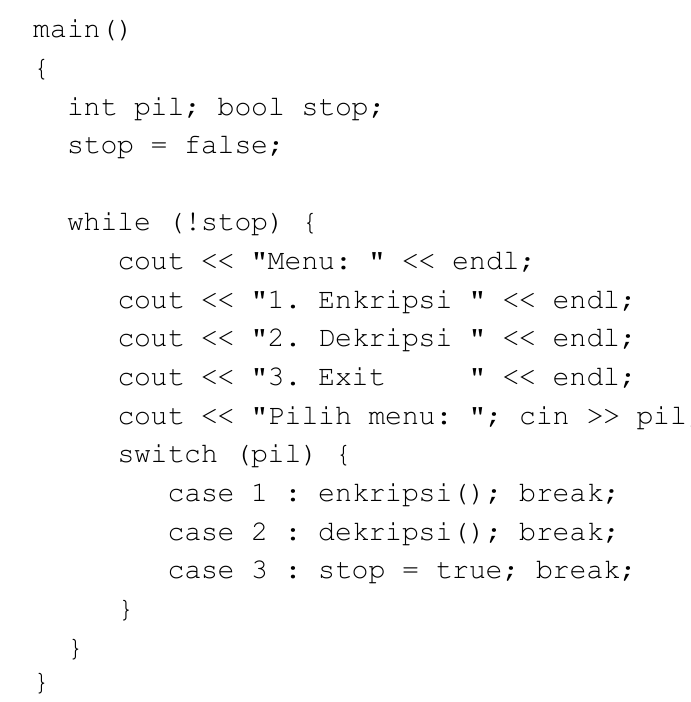
\includegraphics[width=75.60mm,height=193.05mm]{../../images/llm/page_022_img_01.png}%
\end{textblock*}

\end{document}
